\section{Introduction and Objectives}
An individual vehicle observes only part of its surroundings. Buildings,
other vehicles, sensor range, and viewpoint can hide objects that another
vehicle can see. Cooperative perception addresses this limitation by combining
information from multiple observers. The central question is which
information to exchange and how to use it without making computation and
communication costs impractical.

Figure~\ref{fig:occlusion} gives the motivating example used in the project
presentation. Vehicle A follows a truck and obtains returns from its rear
surface. Vehicle B has another line of sight and observes a car farther
ahead. Combining observations makes that complementary information
available to the receiver. This geometric example motivates cooperation;
DiscoNet implements it by exchanging features extracted from the observations.

\begin{figure}[htbp]
\centering
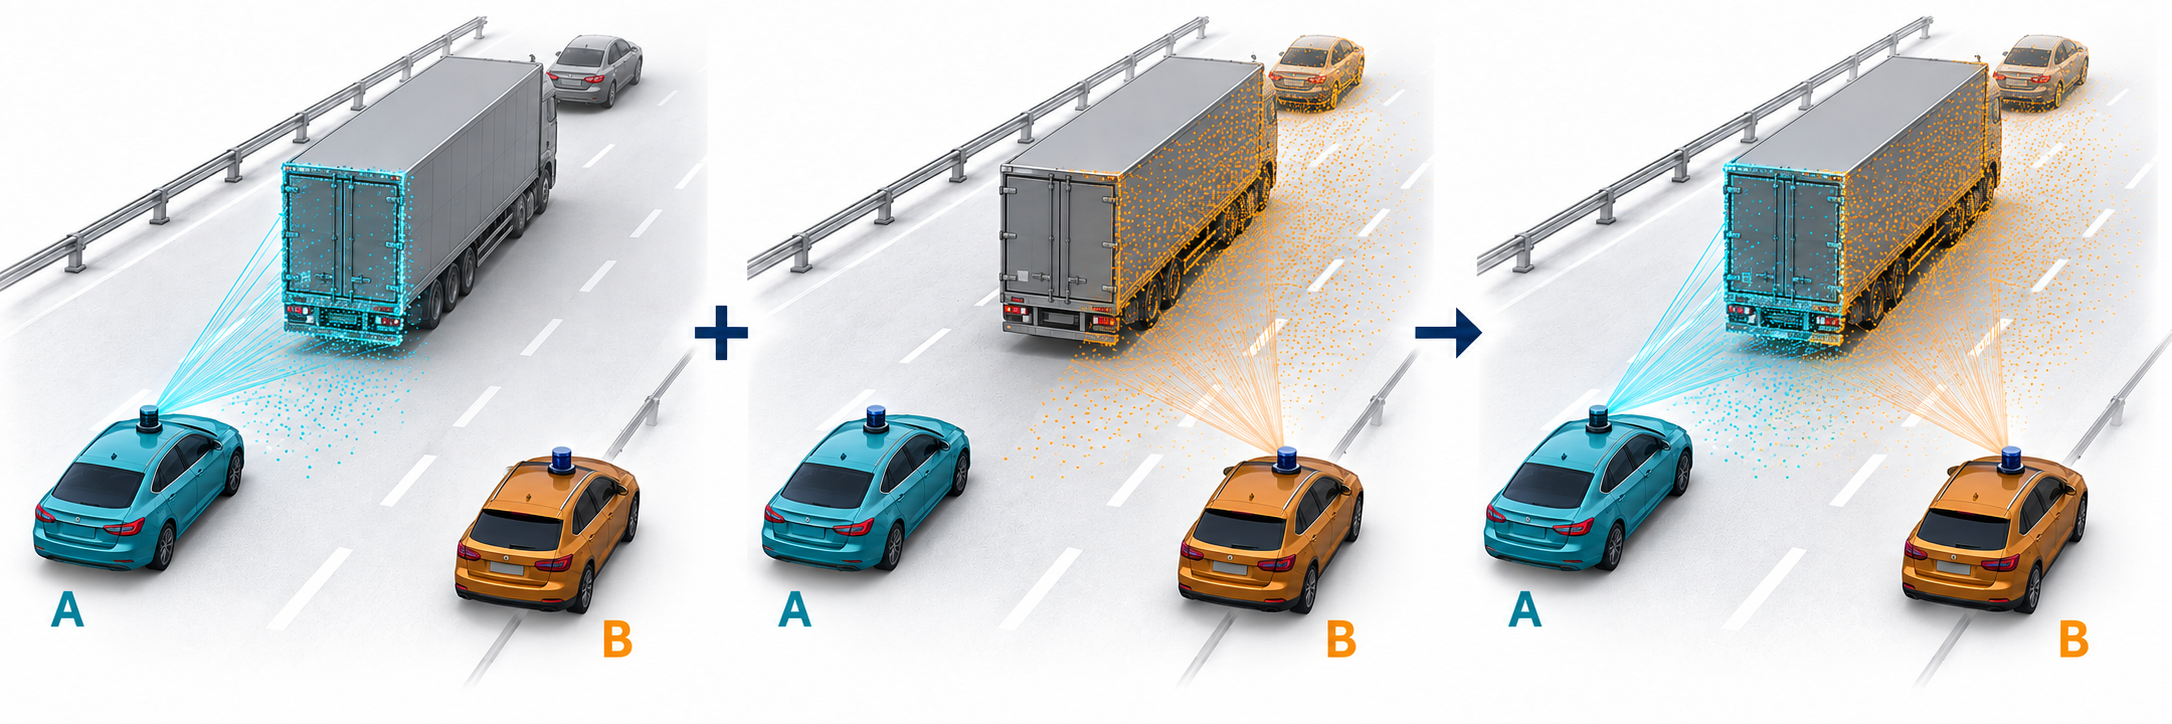
\includegraphics[width=\linewidth]{illustrations/lidar-cooperation-v2.png}
\caption[Complementary observations around an occluding truck]{Project
illustration of complementary LiDAR observations. Cyan and orange distinguish
the two observers; the final panel combines their information. The gray car
ahead of the truck is scene context in the first panel. This is the original
AI-assisted illustration used in the presentation.}
\label{fig:occlusion}
\end{figure}

DiscoNet, introduced by Li et al.~\cite{li2021disconet}, learns spatially
weighted collaboration between agents. This project examines that method
through its architecture and recorded evaluations, rather than developing or
training a detector from scratch. It addresses three questions:
\begin{enumerate}
  \item How are individual LiDAR observations transformed into cooperative
    object detections?
  \item How much does feature sharing improve detection for a fixed trained
    student under ideal communication?
  \item How does execution time grow with the number of model inputs, and
    what changes when fine-resolution collaboration is restricted to a tree?
\end{enumerate}

The original proposal planned a comparison of own-scan perception, early
fusion, and DiscoNet. The completed evidence supports a narrower accuracy
comparison: the same DiscoNet student is evaluated with information sharing
disabled and enabled. Early fusion is explained as the teacher's training
strategy, but no measured early-fusion baseline is available in these results.
The sparse-tree experiment is an additional inference-time ablation of the
released student; it introduces no new training or updated weights.

This study combines the architectural analysis and recorded evidence
presented in the final project slides~\cite{recordslides}. It specifies the
evaluation units and analyzes three distinct experiments. The
full-test benchmark measures detection quality across all active vehicle
views. A separate 30-frame workload measures runtime through 20 input slots.
A matched 30-frame Original/Tree experiment measures runtime and ego-vehicle
AP through 15 slots. These evidence sets are kept separate throughout.

\subsection{Scope and Communication Assumptions}
All conditions assume synchronized observations, accurate relative vehicle
poses, no packet loss, and no communication delay. Agents are evaluated on a
single computer with one GPU. Therefore, a model input slot represents an
agent's data within that computation, not a physically distributed process.
Measured runtime describes the implementation on the recorded hardware; it
does not include a wireless network or establish an end-to-end vehicle
communication latency.

\begin{figure}[htbp]
\centering
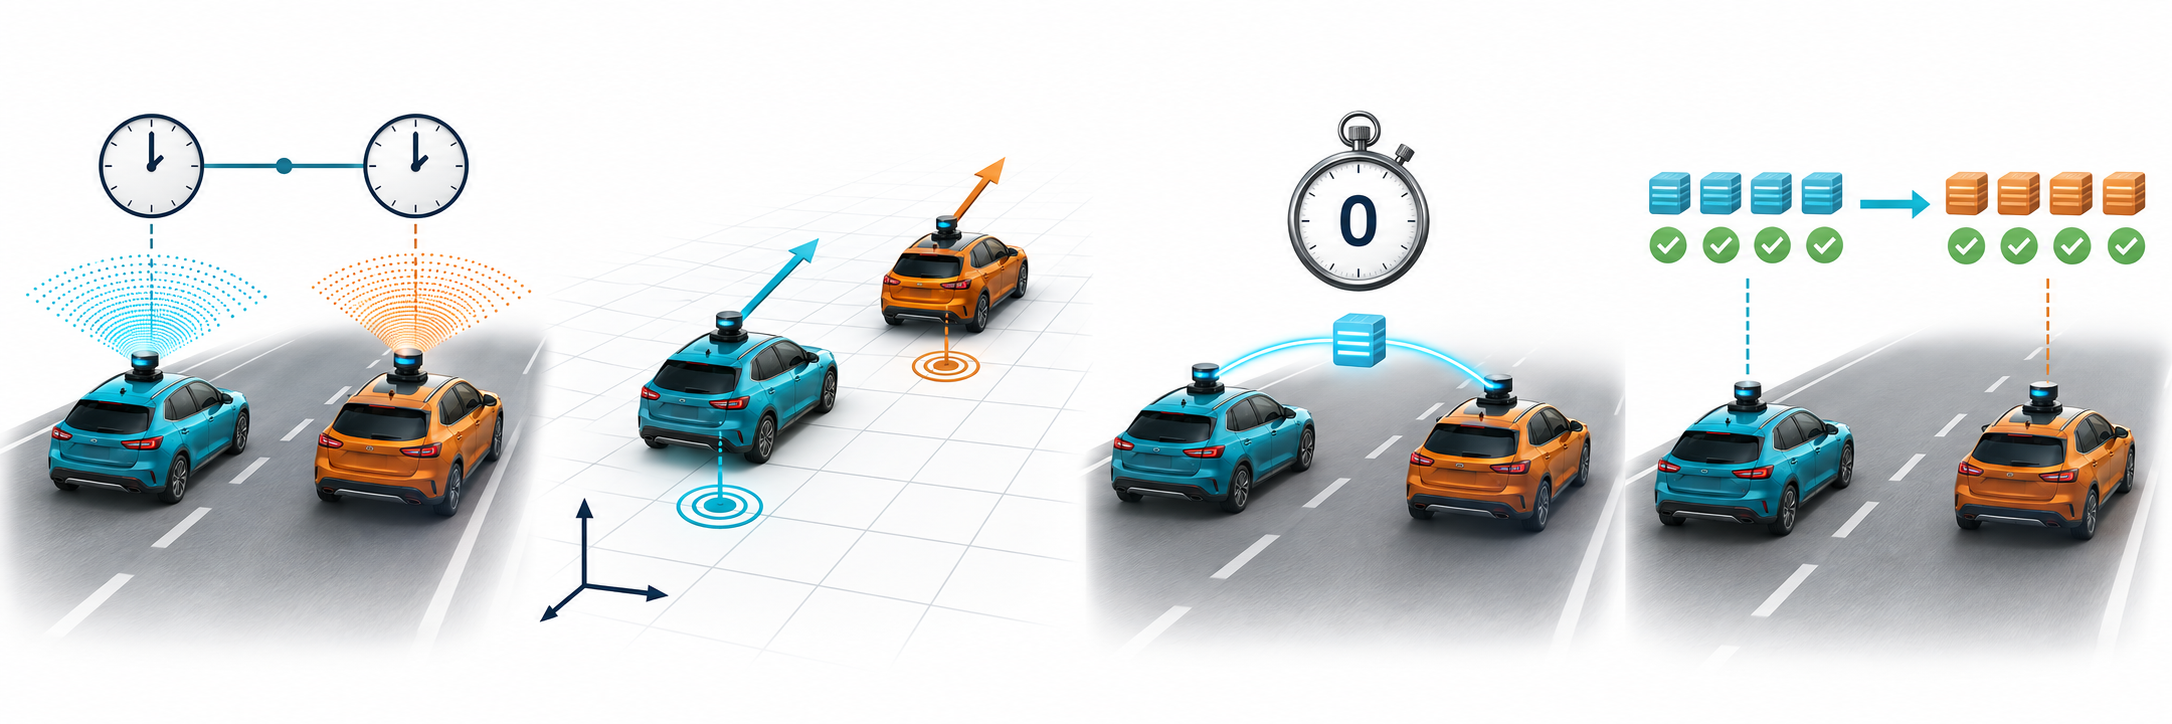
\includegraphics[width=\linewidth]{illustrations/perfect-communication.png}
\caption[The project's ideal communication assumptions]{Project illustration
of the four ideal conditions: synchronized observations, known poses,
zero assumed transmission delay, and complete packet delivery. The clocks,
poses, and packet symbols are explanatory artwork.}
\label{fig:communication-assumptions}
\end{figure}

Figure~\ref{fig:communication-assumptions} summarizes what perfect
communication means in this study. Synchronization makes observations
refer to the same instant, and relative poses allow their feature maps to
be expressed in one coordinate system. Complete delivery means the model
receives the selected inputs without dropped messages. Under these
conditions, the experiments can concentrate on feature fusion and its
computational cost.

\subsection{Organization and Visual Material}
The report follows the path from local observations to cooperative
detections, then explains how those detections and their execution cost
were evaluated. The architecture figures developed for the project expose
individual tensor transformations. The worked metric and convolution
examples make the numerical operations explicit. Recorded detection
overlays, camera views, and quantitative plots then connect that explanation
to the experiment evidence.

Existing project figures are reused throughout, including AI-assisted
conceptual illustrations and vector diagrams~\cite{recordfigures}. Captions
identify teaching examples and recorded results. The additional figure
snapshots and their source hashes are bundled with this report, so the
illustrated explanation remains available with the document sources.
